\documentclass[margin=0px]{article}

\usepackage{listings}
\usepackage[utf8]{inputenc}
\usepackage{graphicx}
\usepackage{float}
\usepackage[magyar]{babel}
\usepackage[a4paper, margin=1in]{geometry}
\usepackage{subcaption}
\usepackage{amsthm}
\usepackage{amssymb}
\usepackage{amsmath}
\usepackage{fancyhdr}
\usepackage[thinlines]{easytable}
\usepackage{hhline}
\usepackage{multirow}
\usepackage[table,xcdraw]{xcolor}
\usepackage[normalem]{ulem}
\usepackage{makecell}
\usepackage{enumitem}
\usepackage{xcolor}
\usepackage[export]{adjustbox}
\usepackage{ifthen}
\usepackage{pgf,tikz}
\usetikzlibrary{positioning,calc,shapes.multipart,arrows,arrows.meta,matrix,automata}

\usepackage{geometry}
 \geometry{
 a4paper,
 total={170mm,297mm},
 left=20mm,
 right=20mm,
 top=20mm,
 bottom=20mm
 }

\renewcommand{\figurename}{ábra}
\newenvironment{tetel}[1]{\paragraph{#1 \\}}{}
\renewcommand{\baselinestretch}{1.15}

\newcommand{\N}{\mathbb{N}}
\newcommand{\Z}{\mathbb{Z}}
\newcommand{\R}{\mathbb{R}}
\newcommand{\Q}{\mathbb{Q}}
\newcommand{\C}{\mathbb{C}}

\definecolor{mygray}{rgb}{0.0, 0.0, 0.0}
\definecolor{blue(pigment)}{rgb}{0.2, 0.2, 0.6}
\definecolor{brickred}{rgb}{0.8, 0.25, 0.33}
\definecolor{coolblack}{rgb}{0.0, 0.18, 0.39}

\setlist[itemize,1]{label=$\bullet$}
\setlist[itemize,2]{label=$\circ$}
\setlist[itemize,3]{label=$\centerdot$}
\setlist[itemize,4]{label=$\bullet$}

\date{}
\useunder{\uline}{\ul}{}
\fancyhf{} % sets both header and footer to nothing
    \lfoot{ELTE-IK}
    \cfoot{\thepage}
    \rfoot{14. tétel }

\pagestyle{fancy}

\renewcommand{\headrulewidth}{0pt}
\renewcommand{\footrulewidth}{0.4pt}


\tikzstyle{pointer}=[fill=black, circle, minimum width = 3pt, inner sep=0]
\tikzstyle{link}=[>=stealth]
\tikzstyle{array}=[draw, fill=green!40, minimum width = 7mm, minimum height = 7mm]
\tikzstyle{list_node_horizontal}=[draw, rectangle split, rectangle split parts=2, rectangle split horizontal,
					rounded corners=2pt,minimum height=5mm, minimum width=10mm, node distance=5mm,fill=red!35]
\tikzstyle{nil}=[draw, rectangle,minimum height=4mm, minimum width=4mm, node distance=5mm]

\tikzset{
node of list/.style = {
             draw,
             minimum height=6mm,
             minimum width=6mm,
             node distance=6mm
   },
link/.style = {
     -stealth,
     shorten >=1pt
     },
array element/.style = {
    draw, fill=white,
    minimum width = 6mm,
    minimum height = 10mm
  },
}

\def\LinkedList#1{%
  \foreach \element [count=\xi] in \list {
     \node[node of list, right = of aux, name=ele] {\element};
     \node[node of list, name=aux2, anchor=west] at ([xshift=-.4pt] ele.east) {};
     \draw[link] (aux) -- (ele);
     \coordinate (aux) at (aux2);
   }
   \ifthenelse{\xi > 0}{
        \node[nil, right = of aux, name=elenil] {};
        \draw (elenil.north east) -- (elenil.south west);
        \draw (elenil.north west) -- (elenil.south east);
        \draw[link] (aux) -- (elenil);
    }
}

\def\Adjacencylist#1{%
  % Draw  Adjacency List
  \foreach [count=\js] \element in \adlist {
	  % a counter the refers to the previous node
	  \prevnode=\j
	  \advance\prevnode by -1
	  % draw the node from the list with a pointer
      \node[list_node_horizontal,right = of node\the\prevnode] (node\js) {\element};
      \path[-] let \p1 = (node\j.two), \p2 = (node\j.center) in
				node[pointer] (rightpointer\js) at (\x1+2,\y2){};
	  %draw incomming link from previous node
      \draw[link,->] (rightpointer\the\prevnode) edge (node\js);
   }
   \node[nil, right = of rightpointer\js] (rightnil) {};
   \draw (rightnil.north east) -- (rightnil.south west);
   \draw (rightnil.north west) -- (rightnil.south east);
   % Draw edge to nil pointer node
   \path [link,->] (rightpointer\js) edge (rightnil);
}
\newcount\prevnode

\begin{document}
    \begin{center}
        {\Large\bfseries\noindent 14. Haladó algoritmusok} \\
    \end{center}

	\section*{Gráfalgoritmusok}
	
    \subsection*{Gráf ábrázolás}

    Legyen a továbbiakban $G = (V, E)$ gráf, ahol
    \begin{itemize}
        \item $V$ a csúcsok halmaza ($|V| = n$),
        \item $E$ pedig a csúcsok közti élek halmaza.
    \end{itemize}

	\paragraph*{Éllistás ábrázolás\\\\}

    \noindent Legyen $G$ véges gráf. Vegyünk fel egy mutatókat tartalmazó $Adj[1...n]$ tömböt (a csúcsokkal indexeljük a tömböt). A tömbben lévő mutatók mutatnak az éllistákra (más néven a szomszédsági listákra). Az éllisták lehetnek egy- vagy kétirányú, fejelemes vagy fejelem nélküli listák, ez most nem lényeges a gráf szempontjából.
    \begin{itemize}
        \item Irányított gráf esetén, az éllisták listaelemei reprezentálják az éleket. Az élnek megfelelő listaelemet abban a listában tároljuk, amelyik csúcsból kiindul az él, és a célcsúcs indexét eltároljuk a listaelemben. Tehát az él megvalósítása az $i$-edik listában egy olyan listaelem, amelyben eltároltuk $j$-t, mint az él célcsúcsát.

        \[
            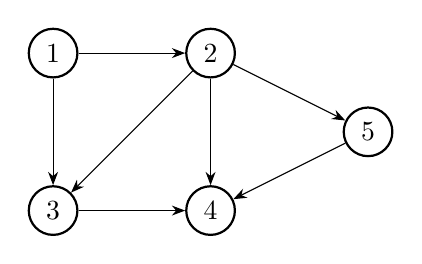
\begin{tikzpicture}[>={Stealth[black]},
                          every node/.style={circle,thick,draw},
                          every edge/.style={draw=red,very thick}]
            %Nodes
                \node (1) at (0,0) {1};
                \node (2) at (2,0) {2};
                \node (3) at (0,-2) {3};
                \node (4) at (2,-2) {4};
                \node (5) at (4,-1) {5};

            %Lines
                \draw[->] (1) -- (2);
                \draw[->] (1) -- (3);
                \draw[->] (2) -- (5);
                \draw[->] (2) -- (3);
                \draw[->] (2) -- (4);
                \draw[->] (3) -- (4);
                \draw[->] (5) -- (4);
            \end{tikzpicture}
            \quad
            % Define graph as a list of pairs, where each pair consists of a node, the delimiter "/" and  the set of adjacent nodes.
            \newcommand{\inputgrapha}{1/{2,3}, 2/{3,4,5}, 3/{4}, 4/{}, 5/{4}}
            \begin{tikzpicture}
            \foreach [count=\i] \index/\list in \inputgrapha {
                \node[array element] (aux) at (0,-\i) {\index};
                \LinkedList{\list}
            }
            \end{tikzpicture}
        \]

        \item Irányítatlan gráf esetén, egy élnek két listaelemet feleltetünk meg, azaz egy irányított élt egy oda-vissza mutató, irányított élpárral valósítunk meg a korábban említett módon. Élsúlyozott gráf esetén, az él súlyát is a listaelemben fogjuk tárolni.

        \[
            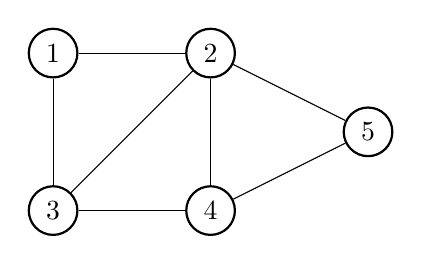
\begin{tikzpicture}[>={Stealth[black]},
                          every node/.style={circle,thick,draw},
                          every edge/.style={draw=red,very thick}]
            %Nodes
                \node (1) at (0,0) {1};
                \node (2) at (2,0) {2};
                \node (3) at (0,-2) {3};
                \node (4) at (2,-2) {4};
                \node (5) at (4,-1) {5};

            %Lines
                \draw[-] (1) -- (2);
                \draw[-] (1) -- (3);
                \draw[-] (2) -- (5);
                \draw[-] (2) -- (3);
                \draw[-] (2) -- (4);
                \draw[-] (3) -- (4);
                \draw[-] (5) -- (4);
            \end{tikzpicture}
            \qquad
            % Define graph as a list of pairs, where each pair consists of a node, the delimiter "/" and  the set of adjacent nodes.
            \newcommand{\inputgraphb}{1/{2,3}, 2/{3,4,1,5}, 3/{1,2,4}, 4/{3,2,5}, 5/{2,4}}
            % Define graph as a list of pairs, where each pair consists of a node, the delimiter "/" and  the set of adjacent nodes.
            \begin{tikzpicture}
            \foreach [count=\i] \index/\list in \inputgraphb {
                \node[array element] (aux) at (0,-\i) {\index};
                \LinkedList{\list}
            }
            \end{tikzpicture}
        \]

    \end{itemize}

    \noindent Az éllistás ábrázolás helyfoglalása irányítatlan gráfok esetén a csúcsok számával (Adj tömb), illetve az élek számával (éllista-elemek száma) arányos. Az elfoglalt memória méretének nagyságrendje ($n + e$). Irányított gráfok esetén az élek számának duplájával kell számolnunk, így ($n + 2e$)-vel arányos helyfoglaláshoz jutunk.

    \noindent Mivel a memóriaigény az élek számával arányos, ezért az éllistás ábrázolást ritka, illetve nem-sűrű (mondhatnánk 'normál') gráfok ($e \ll n^2$) esetén szokták használni, ugyanis sűrű gráf esetén a szomszédsági mátrixhoz képest itt jelentkezik a listák láncolásából származó helyfoglalás is, a mutatók tárolása révén.

	\paragraph*{Szomszédsági mátrix\\\\}

    \noindent Legyen $G = (V, E)$ véges gráf, és $n$ a csúcsok száma. Ekkor a gráfot egy $n \times n$-es mátrixban ábrázoljuk, ahol az oszlopokat és a sorokat rendre a csúcsokkal indexeljük (ez leggyakrabban $1,\ \ldots\ ,n$). Egy mezőben akkor van $1$-es, ha a hozzá tartozó oszlop által meghatározott csúcs szomszédja a sor által meghatározott csúcsnak.
    \[
        C[i,j] = \left\{\begin{array}{lr}
        1, & \text{ha } (i, j) \in E\\
        0, & \text{ha } (i, j) \not\in E\\
        \end{array}\right.
    \]
    Példa:\\\\
    {\footnotesize
    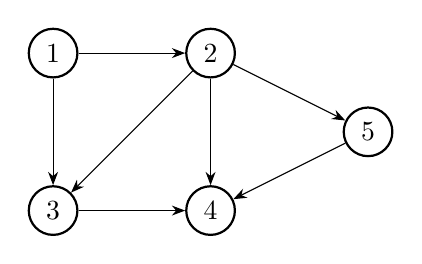
\begin{tikzpicture}[>={Stealth[black]},
                  every node/.style={circle,thick,draw},
                  every edge/.style={draw=red,very thick}]
    %Nodes
        \node (1) at (0,0) {1};
        \node (2) at (2,0) {2};
        \node (3) at (0,-2) {3};
        \node (4) at (2,-2) {4};
        \node (5) at (4,-1) {5};

    %Lines
        \draw[->] (1) -- (2);
        \draw[->] (1) -- (3);
        \draw[->] (2) -- (5);
        \draw[->] (2) -- (3);
        \draw[->] (2) -- (4);
        \draw[->] (3) -- (4);
        \draw[->] (5) -- (4);
    \end{tikzpicture}
    $A^{5 \times 5} = \left[\begin{array}{ccccc}
      0 & 1 & 1 & 0 & 0 \\
      0 & 0 & 1 & 1 & 1 \\
      0 & 0 & 0 & 1 & 0 \\
      0 & 0 & 0 & 0 & 0 \\
      0 & 0 & 0 & 1 & 0
    \end{array}\right]^{5 \times 5} \Leftrightarrow \left[\begin{array}{ccccc}
       \cdot & 1 \rightarrow 2 & 1 \rightarrow 3 & \cdot & \cdot \\
       \cdot & \cdot & 2 \rightarrow 3 & 2 \rightarrow 4 & 2 \rightarrow 5 \\
       \cdot & \cdot & \cdot & 3 \rightarrow 4 & \cdot \\
       \cdot & \cdot & \cdot & \cdot & \cdot \\
       \cdot & \cdot & \cdot & 5 \rightarrow 4 & \cdot
    \end{array}\right]^{5 \times 5}$
    }\\

    \noindent Ha súlyozott a gráf, akkor az élsúlyokat (élköltségeket) is el kell tárolni. Ezt is a mátrixon belül oldjuk meg. A súly valós számokat vehet fel. Természetesen adódik, hogy ahol előzőleg 1-est írtunk, azaz létezett az illető él, oda most írjuk be az él költségét.\\

    \noindent Két további eset maradt, a mátrix főátlója, és az olyan mezők, amelyek esetén nem létezik él. Vezessük be a végtelen ($\infty$) élsúlyt, és a nem létező élek esetén a mátrix megfelelő helyére írjunk $\infty$-t. Egy ilyen "élen" csak végtelen nagy költséggel tudunk végighaladni (tehát nem tudunk).\\

    \noindent A mátrix főátlójába kerülnének a hurokélek költségei, de ilyen értékeket nem alkalmazunk, mivel a legtöbb gyakorlati probléma leírására alkalmas egyszerű gráfokra korlátozzuk. Az egyszerű gráfok nem tartalmaznak hurokéleket (valamint többszörös éleket sem).\\

    \noindent Élsúlyozott gráf esetén a szomszédsági mátrix kitöltését a következő megállapodás szerint végezzük:
    \[
        C[i,j] = \left\{\begin{array}{lr}
        0, & \text{ha } i = j\\
        c(i, j), & \text{ha } (i, j) \in E\\
        \infty, & \text{ha } (i, j) \not\in E\\
        \end{array}\right.
    \]

    \noindent A mátrixos ábrázolás helyfoglalása mindig ugyanakkora, független az élek számától, a mátrix méretével $n^2$-tel arányos. (Az $n$ pontú teljes gráfnak is ekkora a helyfoglalása.) A mátrixos reprezentációt sűrű gráfok esetén érdemes használni, hogy ne legyen túl nagy a helypazarlás.

	\subsection*{Szélességi bejárás}

    A $G$ gráf (irányított/irányítatlan) $s$ startcsúcsából a távolság sorrendjében érjük el a csúcsokat. A legrövidebb utak feszítőfáját adja meg, így csak a távolság számít, a súly nem. A nyilvántartott csúcsokat egy sor adatszerkezetben tároljuk, az aktuális csúcs gyerekeit a sorba tesszük. A következő csúcs pedig a sor legelső eleme lesz. A csúcsok távolságát egy $d$, szüleiket egy $\pi$ tömbbe írjuk, és $\infty$ illetve $0$ értékekkel inicializáljuk.

	\noindent Az algoritmus:
	\begin{enumerate}
		\item Az $s$ startcsúcsot betesszük a sorba
		\item A következő lépéseket addig ismételjük, míg a sor üres nem lesz
        \begin{itemize}
		  \item Kivesszük a sor legelső ($u$) elemét
		  \item Azokat a gyerekcsúcsokat, melyeknek a távolsága nem $\infty$ figyelmen kívül hagyjuk (ezeken már jártunk)
		  \item A többi gyerekre ($v$): beállítjuk a szülőjét ($\pi[v] = u$), a távolságát ($d[v] = d[u]+1$), majd berakjuk a sorba.
        \end{itemize}
	\end{enumerate}

	\subsection*{Minimális költségű utak keresése}

	\paragraph*{Dijkstra algoritmus\\\\}
	
    \noindent Egy $G$ irányított, pozitív élsúlyokkal rendelkező gráfban keres $s$ startcsúcsból minimális költségű utakat minden csúcshoz.\\
					
    \noindent Az algoritmus a szélességi bejárás módosított változata. Mivel itt egy hosszabb útnak lehet kisebb a költsége, mint egy rövidebbnek, egy már megtalált csúcsot nem szabad figyelmen kívül hagyni. Ezért minden csúcs rendelkezik három állapottal (nem elért, elért, kész). A $d$ és $\pi$ tömböket a szélességi bejáráshoz hasonlóan kezeljük.\\
					
	\noindent A még nem kész csúcsokat egy prioritásos sorba helyezzük, vagy minden esetben minimumkeresést alkalmazunk.\\

	\noindent Az algoritmus:
    \begin{enumerate}
        \item Az $s$ startcsúcs súlyát 0-ra állítjuk eltároljuk
        \item A többi csúcs súlyát $\infty$-re állítjuk
		\item A következő lépéseket addig ismételjük, míg a konténerünk üres nem lesz
        \begin{itemize}
            \item Kivesszük a sor legjobb ($u$) elemét, és "kész"-re állítjuk
            \item Ha egy gyerekcsúcs ($v$) nem kész, és a jelenleg hozzávezető út súlya kisebb, mint az eddigi, akkor:\\
            a szülőjét $u$-ra állítjuk ($\pi[v] = u$), és a súlyát frissítjük ($d[v] = d[u]+d(u,v)$).
			\item A többi csúcsot kihagyjuk.
        \end{itemize}
	\end{enumerate}						

    \paragraph*{A minimális költségű utak problémája (negatív élekkel)\\\\}

    \noindent A kezdőcsúcsból elérhető negatív összköltségű körön nem léteznének legkisebb költségű utak, mivel az illető körön tetszőlegesen sokszor végig menve az utak költsége mindig tovább csökkenthető lenne.\\

    \noindent Irányítatlan gráf esetén, egy $(u,v)$ negatív súlyú irányítatlan élen oda-vissza haladva az út költsége szintén korlátlanul csökkenthető lenne, azaz úgy viselkedne, mint egy negatív összköltségű kör. Tekintsük az irányítás nélküli élte tehát negatív összköltségű, két élből álló irányított körnek. Ez egybevág az ábrázolás szintjén megvalósított irányítatlan gráffal, ahol egy irányítatlan élt, egy oda-vissza irányított élpárral valósítunk meg. Tehát irányítatlan gráf esetén a megszorításunk az, hogy egyáltalán ne tartalmazzon negatív súlyú élt, mert az negatív irányított körnek tekinthető.
					
    \paragraph*{Bellman-Ford algoritmus\\\\}

    \noindent Minden csúcsra, ha létezik legrövidebb út, akkor létezik egyszerű legrövidebb út is, mivel a körök összköltsége nem negatív, így a kört elhagyva az út költsége nem nőhet. Egy n pontú gráfban, a legnagyobb élszámú egyszerű út hossza legfeljebb n - 1 lehet.\\

    \noindent A Bellman-Ford-algoritmus a Dijkstra algoritmusnál megismert közelítés műveletét végzi, azaz egy csúcson át a szomszédba vezető él mentén vizsgálja, hogy az illető él része-e a legrövidebb útnak, javító él-e. Egy menetben az összes élre megvizsgálja, hogy javító él-e vagy sem. Összesen n - 1 menetet végez.\\

    
    \noindent Vizsgáljunk meg egy $p^* = s \rightsquigarrow u$ legrövidebb utat. Minden menetben a $p^*$ minden élén végzünk közelítést. Legyen $v \rightarrow w$ él része $p^*$-nak. Miután $p^*$ v-ig tartó részútja $p^*_{v}$ ismertté válik, a következő menetben a $p^*_{v}$ is ismert lesz, mivel az $(v,w)$ éllel is végzünk közelítést. Azonban az élek feldolgozásának (közelítésének) sorrendjére nem tettünk semmilyen megkötést, így csak azt tudjuk garantálni, hogy az első lépés után az 1 élszámú legrövidebb utak, a második lépés után a 2 élszámú legrövidebb utak, és így tovább, válnak ismerté. Mivel a leghosszabb egyszerű út $n - 1$ élszámú, ezért szükséges lehet az $n - 1$ menet.\\

    \noindent Egy $G$ élsúlyozott (akár negatív) irányított gráf $s$ startcsúcsából keres minden élhez minimális költségű utakat, illetve felismeri, ha negatív költségű kör van a gráfban. A $d$ és $\pi$ tömböket az előzőekhez hasonlóan kezeljük.\\
					
	Az algoritmus:
	\begin{enumerate}
    	\item A startcsúcs súlyát állítsuk be 0-ra.
        \item $n-1$ iterációban menjünk végig az összes csúcson, és minden csúcsot ($u$) vessünk össze minden csúccsal ($v$). Ha olcsóbb utat találtunk akkor $v$-be felülírjuk a súlyát ($d[v] = d[u]+d(u,v)$), és a szülőjét ($\pi[v] = u$).
		\item Ha az $n$-edik iterációban is történt módosítás, negatív kör van a gráfban
	\end{enumerate}

	\subsection*{Minimális költségű feszítőfa keresése}

    \noindent A probléma megjelenése egy időszakban, a villamosítás éveiben elég gyakori volt. Ha egy terület villamosítását kell megoldani a lehető legkisebb költséggel, akkor a feladat minimális összköltségű vezetékrendszer tervezése megadott helységek között.\\

    \noindent A modellünk legyen irányítás nélküli, súlyozott gráf, ahol a városoknak megfeleltetjük a gráf pontjait, az éleknek pedig a tervezett, két várost összekötő villamos vezetéket. Az élek irányítás nélküliek az elektromos áram irányítatlan tulajdonsága miatt, és súlyozottak, ahol az élek költségei legyenek a becsült építési költségek.\\
    
    \noindent Legyen $G(V, E)$ irányítatlan gráf.
    \begin{itemize}
        \item Részgráf: A $G' = (V', E')$ gráf, G \textbf{\emph{részgráfja}}, ha $V' \subseteq V$ és $E' \subseteq E$ és $\forall (u, v) \in E': u, v \in V'$.
        \item Feszítőfa: $F = (V, E')$ összeföggő, körmentes irányítatlangráfot G \textbf{\emph{feszítőfájának}} nevezzük.\\
        (F és G csúcshalmaza azonos)
        \item Minimális feszítőfa: $F = (V, E')$ feszítőfa minimális, ha G feszítőfái között az élek költsége 
        \[c(H) = \sum\limits_{(u,v) \in E'}c(u,v)\] 
        minimális, azaz
        \[
            C(F) = \left\{c(H)\ \big|\ \text{\emph{H} feszítőfája \emph{G}-nek}\right\}
        \]
    \end{itemize}

    \paragraph*{Prim-algoritmus\\\\}

    \noindent Egy speciális piros-kék algoritmus, amely minden lépésben a kék szabályt alkalmazza.\\
    
    \noindent \textbf{\emph{Kék szabály}}: Válasszunk ki egy olyan $\emptyset \neq X \subset V$ csúcshalmazt, amiből nem vezet ki kék él. \\
    Ez után egy legkisebb súlyú $X$-ből kimenő szintelen élt fessünk kékre.\\

    \noindent Az algoritmus:
	\begin{itemize}
        \item Válasszuk ki a gráf egy tetszőleges csúcsát, legyen ez egy egy csúcsú fa. (kezdő X)
        \item Ameddig van a gráfnak olyan csúcsa, amelyik nincs benne a fában, végezzük el a következőket:
        \begin{itemize}
            \item Válasszuk ki a fa csúcsai és a gráf többi csúcsa között futó élek közül a legkisebb súlyút.\\
            $min\left\{(u, v) \in E\Big|\ u \in X,\ v \not \in X,\ (u, v) \not \in X\right\}$
            \item A kiválasztott él nem fabeli csúcsát tegyük át a fába az éllel együtt. (kékre festés)
        \end{itemize}
    \end{itemize}
    
	\begin{figure}[H]
		\centering
		\includegraphics[width=0.7\textwidth]{img/spanning_tree.jpg}
		\caption{Prim algoritmus}
		\label{fig:Prim_sample}
	\end{figure}    

	\subsection*{Mélységi bejárás}

    \noindent A mélységi bejárás kidolgozása felé lépve, megkülönböztetjük a csúcsok státuszát. Erre több, szemléletében különböző módszerrel találkozhatunk, amelyek végső ugyanazt a célt érik el. Itt a színezés eszközével élünk és három színt használunk. Attól függően színezzük a csúcsokat, hogy az illető csúcsot illetően a bejárás milyen fázisban van.\\

    \noindent Egy csúcs legyen fehér, ha még nem jutottunk el hozzá a bejárás során (kezdetben minden csúcs fehér).\\
    \noindent Egy csúcs legyen szürke, ha a bejárás során már elértük a csúcsot, de még nem állíthatjuk, hogy az illető csúcsból elérhető összes csúcsot meglátogattuk.\\
    \noindent A csúcs legyen fekete, ha azt mondhatjuk, hogy az illető csúcsból elérhető összes csúcsot már meglátogattuk és visszamehetünk (vagy már visszamentünk) az idevezető út megelőző csúcsára\\

    \noindent A bejárás során tároljuk el, hogy egy csúcsot hányadikként értünk el, azaz hányadikként lett szürke és tároljuk el azt is, hogy hányadikként fejeztük be a csúcs, és a belőle elérhető csúcsok bejárását, azaz a csúcs hányadikként lett fekete. Az említett számokat nevezzük mélységi, illetve befejezési számnak, amelyeket az ábrákon a csúcsok címkéi alatt jelenítünk meg. (Alternatív szóhasználat: belépési, illetve kilépési számok.) Utalunk arra, hogy ezeknek a számoknak lényeges szerep jut majd az élek osztályozásánál.\\

    \noindent A következő ábrákon egy gráf mélységi bejárása látható. A példában szereplő gráfon a csúcsokból kimenő élek feldolgozási sorrendje legyen a rákövetkező csúcsok címkéje szerint növekedően, vagyis alfabetikusan rendezett (például a láncolt ábrázolásnál az éllista a csúcsok címkéje szerint rendezett).\\

    Nézzük az első ábrát, amelyben a kezdőcsúcs legyen az 1-es csúcs. Legyen kezdetben minden csúcs fehér, és a mélységi és befejezési számuk is legyen az extremális 0. A kezdőcsúcsot érjük el elsőként, tehát színezzük szürkére, és a mélységi számát állítsuk be 1-re.\\

	\begin{figure}[H]
		\centering
		\includegraphics[width=0.9\textwidth]{img/melysegi_1.png}
		\label{fig:melysegi_pelda_1}
	\end{figure}    

    \noindent Az 1-es csúcsból három él vezet ki, de a kikötöttük, hogy az élek feldolgozási sorrendje legyen a szomszéd csúcsok címkéje szerint növekedően rendezett. Ekkor a 2-es csúcsot érjük el másodikként. Ezután harmadikként a 4-es csúcs, majd negyedikként a 8-as csúcs következik. Mivel a 8-as csúcsnak egyáltalán nincs szomszédja, bejárását befejeztük és a csúcsot feketére színezzük. Mivel a bejárás során a 8-as csúcs lett elsőként fekete, a befejezési száma 1-es lesz.

	\begin{figure}[H]
		\centering
		\includegraphics[width=0.9\textwidth]{img/melysegi_2.png}
		\label{fig:melysegi_pelda_2}
	\end{figure}

    \noindent A bejárás során eddig megtett utunk $<1,2,4,8>$. Most menjünk vissza az utolsó előtti 4-es csúcsra. Mivel a 4-es csúcsnak sincs meg nem látogatott szomszédja, így ennek csúcs bejárását is befejeztük; színezzük a csúcsot feketére, és a bejárási számát állítsuk 2-re.\\
    Menjünk vissza a 2-es csúcshoz. A 2-es csúcsnak két olyan szomszédja is van, amelyet még nem látogattunk meg. Lépjünk a kisebb címkéjű csúcsba.\\
    Az 5-ös csúcs bejárását harmadikként fejezzük be. A 2-es csúcsból a bejárást a 6-os csúcs irányába folytatjuk.\\
    Tovább haladva, hetedikként elérjük a 9-es csúcsot. Nyolcadikként következik a 7-es csúcs. Mivel a 3-as csúcs még fehér, azt érjük el kilencedikként

	\begin{figure}[H]
		\centering
		\includegraphics[width=0.9\textwidth]{img/melysegi_3.png}
		\label{fig:melysegi_pelda_3}
	\end{figure}

    \noindent A 3-as csúcsból a 6-os csúcsba vezet él, azonban a 6-os csúcsot már bejártuk, a színe már nem fehér, erre már nem folytatjuk a bejárást. \\
    Mivel a 3-as csúcsból már nem vezet él fehér csúcsba, így a 3-as csúcs bejárását is befejeztük.\\
    Visszamegyünk a 7-es csúcsba, ahol a sorrendben következő él, a $(7,8)$ mentén látjuk, hogy a 8-as csúcs színe már fekete. Mivel a 7-es csúcsnak nincs fehér szomszédja, így ötödikként befejeztük a bejárását.\\
    A 9-es csúcsnak a bejárását is befejeztük. Az úton ismét egy csúccsal visszamegyünk és befejezzük a 6-os csúcsot.\\
    A 2-es csúcsra lépve, látható, hogy minden kimenő éle mentén már próbálkoztunk, így nyolcadikként azt is elhagyjuk.

	\begin{figure}[H]
		\centering
		\includegraphics[width=0.9\textwidth]{img/melysegi_4.png}
		\label{fig:melysegi_pelda_4}
	\end{figure}


%    \noindent Legyen $G = (V,E)$ irányított vagy irányítatlan véges gráf, ahol $V = \{1, 2, \ldots, n\}$.\\
%    Továbbá, definiáljuk az alábbi tömböket:
%    \begin{itemize}
%        \item szín[1...n]: az ADS szintű színezés megvalósítására
%        \item mszám[1...n] és bszám[1...n]: mélységi és befejezési számok
%        \item $\pi[1\ldots n]$: a bejárás során, egy csúcs megelőző csúcsának a nyilvántartására.
%    \end{itemize}

    \paragraph*{A mélységi bejárás algoritmusa\\\\}

    \noindent Az előző példában úgy kezdtük a bejárást, hogy kijelöltünk egy kezdőcsúcsot, amelyből kiindulva történetesen az összes csúcs elérhető volt mélységi bejárással. Egy másik példában előfordulhatna, hogy lennének olyan csúcsok, amelyeket egyáltalán nem tudnánk elérni egy kiválasztott startcsúcsból. A későbbi alkalmazások érdekében a mélységi bejárást úgy definiáljuk, hogy az a gráf minden pontjához eljusson.\\

    \noindent Az algoritmus működésének nem feltétele egy kezdőcsúcs megadása, azt az eljárás keretében magunk tetszőlegesen választjuk meg, kívülről nézve véletlen jelleggel. Miután minden, ebből elérhető csúcsot bejártunk, visszajutottunk az említett kezdőpontba. Ha maradt olyan csúcs, amelyet a bejárás nem ért el, azaz színe fehér maradt, akkor választunk közülük egy következőt és abból kiindulva újra elvégezzük a mélységi bejárást.\\

    \noindent Ezt az eljárást addig folytatjuk, amíg van fehér csúcsunk. Nyilván minden ilyen menetben legalább egy csúcsot átszínezünk feketére, tehát véges számú menet után elfogynak a fehér csúcsok. Elegendő a csúcsok halmazán egyszer végigmenni (a gyakorlatban a csúcsok címkéje szerinti növekedően), és ha egy csúcs színe fehér, akkor onnan indítsunk egy bejárást.\\
	
    \noindent A gráf éleit a mélységi bejárás közben osztályozhatjuk. (Inicializáláskor minden értéket 0-ra állítottunk)
    \begin{itemize}
        \item Faél: A következő csúcs mélységi száma = 0
        \item Visszaél: A következő csúcs mélységi száma $ > 0$, és befejezési száma $= 0$\\
        (Tehát az aktuális út egy előző csúcsára kanyarodunk vissza)
        \item Keresztél: A következő csúcs mélységi száma $ > 0$, és befejezési száma $ > 0$, továbbá az aktuális csúcs mélységi száma $>$ következő csúcs mélységi száma.\\
        (Ekkor egy az aktuális csúcsot megelőző csúcsból induló, már megtalált útba mutató éllel van dolgunk)
        \item Előreél: A következő csúcs mélységi száma $ > 0$, és befejezési száma $ > 0$, továbbá az \\
        aktuális csúcs mélységi száma $ < $ következő csúcs mélységi száma.\\
        (Ekkor egy az aktuális csúcsból induló, már megtalált útba mutató éllel van dolgunk)
	\end{itemize}
	
    \subsection*{DAG Topologikus rendezése\\}

	\paragraph*{Alapfogalmak}

	\begin{itemize}
        \item Topologikus rendezés
        Egy $G(V,E)$ gráf topologikus rendezése a csúcsok olyan sorrendje, melyben \\
        $\forall (u\rightarrow v) \in E$ élre $u$ előbb van a sorrendben, mint $v$
        \item DAG - Directed Acyclic Graph
            Irányított körmentes gráf. \\
            Legtöbbször munkafolyamatok irányítására illetve függőségek analizálására használják.
							
			Tulajdonságok:
			\begin{itemize}
                \item Ha $G$ gráfra a mélységi bejárás visszaélt talál (Azaz kört talált) $\Longrightarrow$ $G$ nem DAG
				\item Ha $G$ nem DAG (van benne kör) $\Longrightarrow$ Bármely mélységi bejárás talál visszaélt
                \item Ha $G$-nek van topologikus rendezések $\Longrightarrow$ $G$ DAG
                \item Minden DAG topologikusan rendezhető.
            \end{itemize}
	\end{itemize}
	\paragraph*{DAG topologikus rendezése\\}

    Egy $G$ gráf mélységi bejárása során tegyük verembe azokat a csúcsokat, melyekből visszaléptünk. Az algoritmus után a verem tartalmát kiírva megkapjuk a gráf egy topologikus rendezését.

	\section*{Adattömörítések}

	\subsection*{Huffman-algoritmus}

    \noindent A Huffman-kódolás karakterek (jelek, betűk, számjegyek) olyan kódolását jelenti, ahol az egyes karakterekhez rendelt kódok nem azonos hosszúságúak (különböző számú bitből állnak), így a belőlük alkotott szöveg hosszában rövidíthetővé válik. Ez a karakterek gyakoriságának figyelembevételével történik. Maga a kódolás egy mohó stratégián alapszik, és az adattömörítésben igen hatékonyan használható.\\

    \noindent A kódolás során egy speciális adatszerkezetet (lényegében egy bináris fát, amely most egyszerűen csak listaként ábrázolunk) építünk fel lépésről-lépésre, a következő módon:

    \begin{enumerate}
        \item Kiválasztjuk a lista két legkisebb gyakoriságú elemét, amely egy háromcsúcsú bináris fa két levele (olyan csúcs, amelynek nincs gyereke) lesz (amelyeket a gyakorisággal címkézzük meg), majd ezekhez hozzárendelünk egy gyökeret, amelyet a két gyakoriság összegével címkézünk meg.

        \item Ezután a két vizsgált elemet kitöröljük a listából, és azok összegét beszúrjuk az érték szerinti megfelelő helyre, hogy a lista rendezettsége megmaradjon.

        \item Ezután folytatjuk a műveletet az 1. lépésnél mindaddig, amíg van elem a listában.
    \end{enumerate}

    \noindent Az így felépített adatszerkezetben a levelek az eredeti karaktereknek (illetve azok gyakoriságának) felelnek meg.\\

    \noindent Az eredményül kapott fában, minden csúcs esetében címkézzük meg 0-val a belőle kiinduló bal oldali élt, 1-gyel pedig a jobb oldalit.\\

    \noindent A gyökértől egy adott levélig egyetlen út halad. Ezen út éleihez rendelt 0 és 1 címkéket sorrendben összeolvasva, megkapjuk a levélhez rendelt karakter kódját. Látható, hogy a gyakoribb karakterek kódja rövidebb, míg a kevésbé gyakoribbaké hosszabb lesz.\\

    \noindent Megjegyzés: Attól függően, hogy a bináris fa felépítésében egy adott lépésben melyik elem kerül balra és melyik jobbra, különböző eredményt kaphatunk, de ez nem befolyásolja a kapott kód hatékonyságát, illetve a megoldás helyességét.\\
			
	\noindent Példa: Legyen a következő öt betű, mely a megadott gyakorisággal fordul elő (már növekvő sorrendben):\\\\
    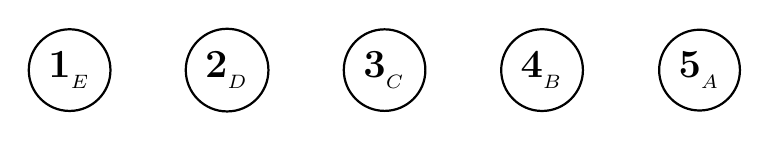
\begin{tikzpicture}[->,>=stealth',shorten >=1pt,auto,node distance=4cm,
                thick,main node/.style={circle,draw,font=\Large\bfseries}]
%Nodes
    \node[main node] (E1) at (0,0) {$\textbf{1}_{_{E}}$};
    \node[main node] (D1) at (2,0) {$\textbf{2}_{_{D}}$};
    \node[main node] (C1) at (4,0) {$\textbf{3}_{_{C}}$};
    \node[main node] (B1) at (6,0) {$\textbf{4}_{_{B}}$};
    \node[main node] (A1) at (8,0) {$\textbf{5}_{_{A}}$};
%Lines
\end{tikzpicture}\\
			
	\noindent Ekkor a redukciós lépések a következők:\\
			
    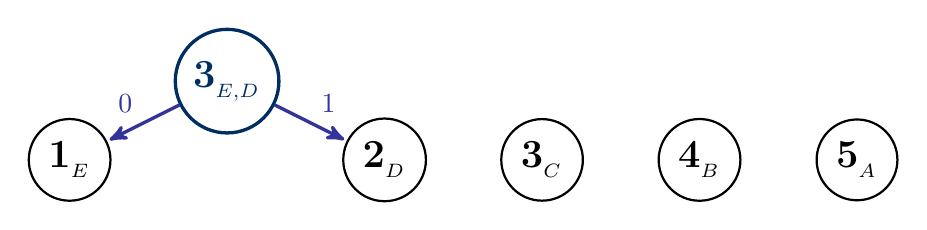
\begin{tikzpicture}[->,>=stealth',shorten >=1pt,auto,node distance=4cm,
                thick,main node/.style={circle,draw,font=\Large\bfseries}]
%Nodes
    \node[main node] (E1) at (-2,-1) {$\textbf{1}_{_{E}}$};
    \node[main node] (D1) at (2,-1) {$\textbf{2}_{_{D}}$};
    \node[main node, color=coolblack, very thick] (ED1) at (0,0) {$\textbf{3}_{_{E,D}}$};
    \node[main node] (C1) at (4,-1) {$\textbf{3}_{_{C}}$};
    \node[main node] (B1) at (6,-1) {$\textbf{4}_{_{B}}$};
    \node[main node] (A1) at (8,-1) {$\textbf{5}_{_{A}}$};

    \draw[->, color=blue(pigment), very thick] (ED1) edge node[above left] {0} (E1);
    \draw[->, color=blue(pigment), very thick] (ED1) edge node {1} (D1);
\end{tikzpicture}\\\\
			
    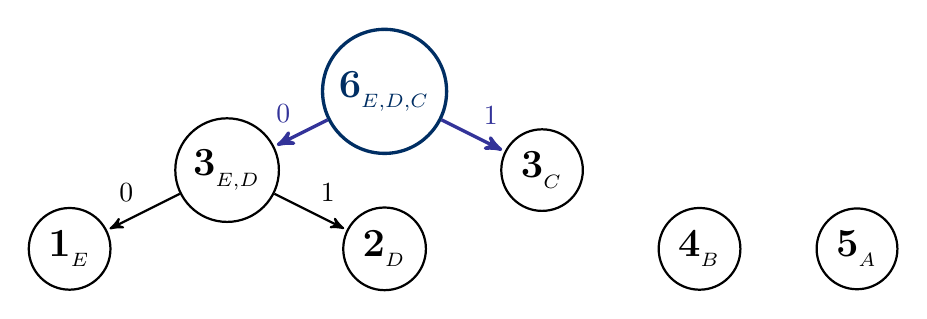
\begin{tikzpicture}[->,>=stealth',shorten >=1pt,auto,node distance=4cm,
                thick,main node/.style={circle,draw,font=\Large\bfseries}]
%Nodes
    \node[main node] (E1) at (-2,-1) {$\textbf{1}_{_{E}}$};
    \node[main node] (D1) at (2,-1) {$\textbf{2}_{_{D}}$};
    \node[main node] (ED1) at (0,0) {$\textbf{3}_{_{E,D}}$};
    \node[main node] (C1) at (4,0) {$\textbf{3}_{_{C}}$};
    \node[main node, color=coolblack, very thick] (ECD1) at (2,1) {$\textbf{6}_{_{E,D,C}}$};
    \node[main node] (B1) at (6,-1) {$\textbf{4}_{_{B}}$};
    \node[main node] (A1) at (8,-1) {$\textbf{5}_{_{A}}$};

    \draw[->] (ED1) edge node[above left] {0} (E1);
    \draw[->] (ED1) edge node {1} (D1);
    \draw[->, color=blue(pigment), very thick] (ECD1) edge node[above left] {0} (ED1);
    \draw[->, color=blue(pigment), very thick] (ECD1) edge node {1} (C1);
\end{tikzpicture}\\\\
				
    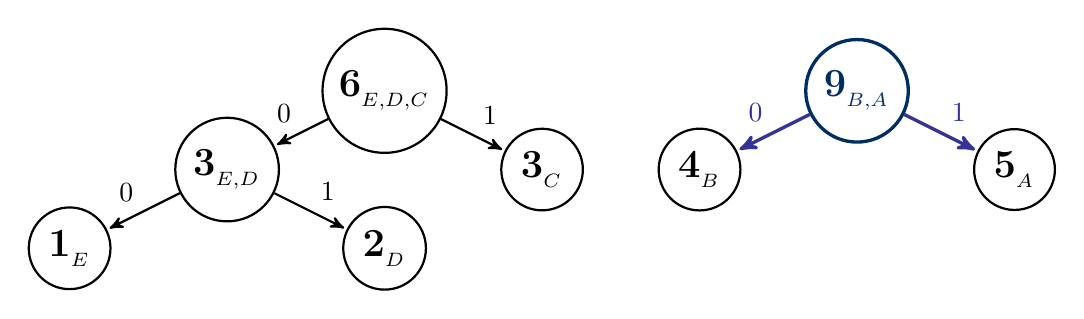
\begin{tikzpicture}[->,>=stealth',shorten >=1pt,auto,node distance=4cm,
                thick,main node/.style={circle,draw,font=\Large\bfseries}]
%Nodes
    \node[main node] (E1) at (-2,-1) {$\textbf{1}_{_{E}}$};
    \node[main node] (D1) at (2,-1) {$\textbf{2}_{_{D}}$};
    \node[main node] (ED1) at (0,0) {$\textbf{3}_{_{E,D}}$};
    \node[main node] (C1) at (4,0) {$\textbf{3}_{_{C}}$};
    \node[main node] (ECD1) at (2,1) {$\textbf{6}_{_{E,D,C}}$};
    \node[main node, color=coolblack, very thick] (BA1) at (8,1) {$\textbf{9}_{_{B,A}}$};
    \node[main node] (B1) at (6,0) {$\textbf{4}_{_{B}}$};
    \node[main node] (A1) at (10,0) {$\textbf{5}_{_{A}}$};

    \path[->] (ED1) edge node[above left] {0} (E1);
    \path[->] (ED1) edge node {1} (D1);
    \path[->] (ECD1) edge node[above left] {0} (ED1);
    \path[->] (ECD1) edge node {1} (C1);
    \path[->, color=blue(pigment), very thick] (BA1) edge node[above left] {0} (B1);
    \path[->, color=blue(pigment), very thick] (BA1) edge node {1} (A1);
\end{tikzpicture}\\\\

    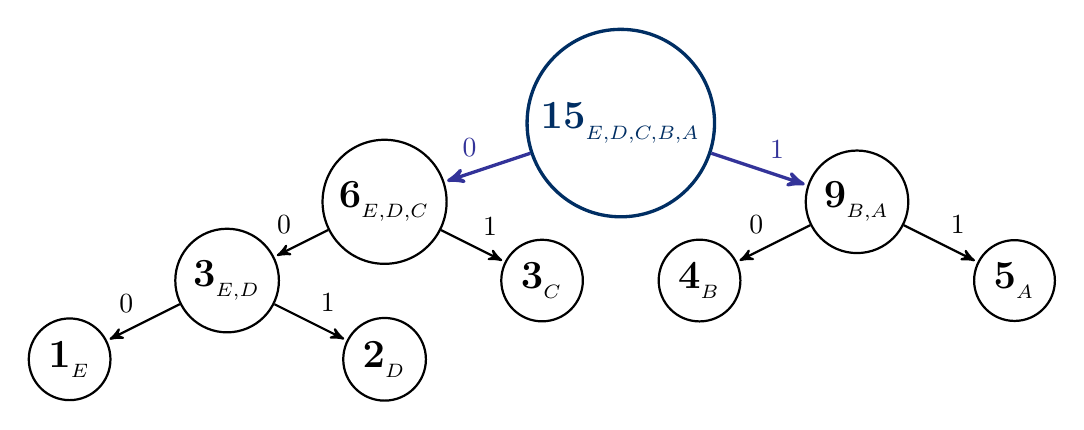
\begin{tikzpicture}[->,>=stealth',shorten >=1pt,auto,node distance=4cm,
                thick,main node/.style={circle,draw,font=\Large\bfseries}]
%Nodes
    \node[main node] (E1) at (-2,-1) {$\textbf{1}_{_{E}}$};
    \node[main node] (D1) at (2,-1) {$\textbf{2}_{_{D}}$};
    \node[main node] (ED1) at (0,0) {$\textbf{3}_{_{E,D}}$};
    \node[main node] (C1) at (4,0) {$\textbf{3}_{_{C}}$};
    \node[main node] (ECD1) at (2,1) {$\textbf{6}_{_{E,D,C}}$};
    \node[main node] (BA1) at (8,1) {$\textbf{9}_{_{B,A}}$};
    \node[main node] (B1) at (6,0) {$\textbf{4}_{_{B}}$};
    \node[main node] (A1) at (10,0) {$\textbf{5}_{_{A}}$};
    \node[main node, color=coolblack, very thick] (ECDBA1) at (5,2) {$\textbf{15}_{_{E,D,C,B,A}}$};

    \path[->] (ED1) edge node[above left] {0} (E1);
    \path[->] (ED1) edge node {1} (D1);
    \path[->] (ECD1) edge node[above left] {0} (ED1);
    \path[->] (ECD1) edge node {1} (C1);
    \path[->] (BA1) edge node[above left] {0} (B1);
    \path[->] (BA1) edge node {1} (A1);
    \path[->, color=blue(pigment), very thick] (ECDBA1) edge node[above left] {0} (ECD1);
    \path[->, color=blue(pigment), very thick] (ECDBA1) edge node {1} (BA1);
\end{tikzpicture}\\
			
    \noindent Tehát a kódszavak:\\
			
	\begin{tabular}{|c|c|c||c|c|}
		\hline A & B & C & D & E \\
		\hline 11 & 10 & 01 & 001 & 000 \\
		\hline
	\end{tabular}\\
\newpage
    \subsection*{LZW-algoritmus}

    Az LZW (Lempel-Ziv-Welch) egy veszteségmentes tömörítési algoritmus. A tömörítésnek a lényege, hogy egy szótárat bővítünk folyamatosan, és az egyes kódolandó szavakhoz szótárindexeket rendelünk.

	\paragraph*{Kódolás\\\\}

    A kódolás algoritmusa a következő lépésekből áll:
	\begin{enumerate}
		\item A szótárt inicializáljuk az összes 1 hosszú szóval
		\item \label{itm:szotar} Kikeressük a szótárból a leghosszabb, jelenlegi inputtal összeillő $W$ sztringet
		\item $W$ szótárindexét kiadjuk, és $W$-t eltávolítjuk az inputról
		\item A $W$ szó és az input következő szimbólumának konkatenációját felvesszük a szótárba
		\item A \ref{itm:szotar}. lépéstől ismételjük
	\end{enumerate}

    \noindent Példa:\\\\
            \textbf{{\color{blue(pigment)}B}}emenet: wabbawabba\\\\
            \textbf{{\color{blue(pigment)}S}}zótár:
            $\begin{array}{|c|c|c||c|c|c|c|c|c|c|}
              a & b & w & wa & ab & bb & ba & aw & wab & bba\\ \hline
              1 & 2 & 3 & 4 & 5 & 6 & 7 & 8 & 9 & 10
            \end{array}$\\\\

            \small
            \noindent \begin{tabular}{|c|c|c|c|c|}
              \hline
              % after \\: \hline or \cline{col1-col2} \cline{col3-col4} ...
              \text{\textbf{{\color{blue(pigment)}I}}ndex} & \makecell{ \text{\textbf{{\color{blue(pigment)}E}}lőző} \\ $ \left\{
                \begin{array}{lr}
                    \textbf{B[I-1]},\ \text{ha}\ E + J \in S \wedge I \geq 2\\
                    \textbf{E} + \textbf{B[I-1]},\ \text{ha}\ K[I-1] = \varnothing \wedge I \geq 2\\
                    \varnothing,\ \text{különben}\
                \end{array} \right.$ } & \makecell{ \text{\textbf{{\color{blue(pigment)}J}}elenlegi}\\ B[I] } & \makecell { \small \text{\textbf{{\color{blue(pigment)}K}}ód}\\ $ \left\{
                \begin{array}{lr}
                    \textbf{E} + \textbf{J},\ \text{ha}\ E + J \not\in S\\
                    \varnothing,\ \text{ha}\ E + J \in S
                \end{array} \right.$ } & \makecell { \text{\textbf{{\color{blue(pigment)}K}}imenet} \\ $\left\{
                \begin{array}{lr}
                    \textbf{E},\ \text{ha}\ \text{K} \neq \varnothing \vee J = \varnothing \\
                    \varnothing,\ \text{ha}\ \text{K} = \varnothing
                \end{array} \right. $ } \\ \hline
              1 & & w &   &  \\  \hline
              2 & w & a & wa - 4 & $\textbf{3}$ \\  \hline
              3 & a & b & ab - 5 & $\textbf{1}$ \\  \hline
              4 & b & b & bb - 6 & $\textbf{2}$ \\  \hline
              5 & b & a & ba - 7 & $\textbf{2}$ \\  \hline
              6 & a & w & aw - 8 & $\textbf{1}$ \\  \hline
              7 & w & a & &  \\  \hline
              8 & wa & b & wab - 9 & $\textbf{4}$ \\  \hline
              9 & b & b & &  \\  \hline
              10 & bb & a & bba - 10 & $\textbf{6}$ \\  \hline
              $(11) \oslash$ & a & &  & $\textbf{1}$ \\ \hline
            \end{tabular}\\\\
    Kimenet: 3 1 2 2 1 4 6 1\\

    \paragraph*{Dekódolás\\\\}

    A dekódolás során is építenünk kell a szótárat. Ezt már azonban csak a dekódolt szöveg(rész) segítségével tudjuk megtenni, mivel egy megkapott kód dekódolt szava és az utána lévő szó első karakteréből áll össze a szótár következő eleme.\\
					
	\noindent Tehát a dekódolás lépései:
	\begin{enumerate}
		\item Kikeressük a kapott kódhoz tartozó szót a szótárból ($u$), az output-ra rakjuk
		\item Kikeressük a következő szót ($v$) a szótárból, az első szimbólumát $u$-hoz konkatenálva a szótárba rakjuk a következő indexszel.
		\item Amennyiben már nincs következő szó, dekódolunk, de nem írunk a szótárba.
	\end{enumerate}
					
    \noindent Megtörténhet az az eset, hogy mégis kapunk olyan kódszót, mely még nincs benne a szótárban. Ez akkor fordulhat elő, ha a kódolásnál az aktuálisan szótárba írt szó következik.\\
\newpage						
	\noindent Példa:\\
					
	\noindent Szöveg: AAA\\
	\noindent Szótár: A - 1\\
					
    \noindent Ekkor a kódolásnál vesszük az első karaktert, a szótárbeli indexe 1, ezt kiküldjük az outputra. A következő karakter A, így AA-t beírjuk a szótárba 2-es indexszel. Az első karaktert töröljük az inputról. Addig olvasunk, míg szótárbeli egyezést találunk, így AA-t olvassuk (amit pont az előbb raktunk be), ennek indexe 2, tehát ezt küldjük az outputra. AA-t töröljük az inputról, és ezzel végeztünk is. Az output: 1,2\\
					
    \noindent Dekódoljuk az 1,2 inputot! Jelenleg a szótárban csak A van 1-es indexszel. Vegyük az input első karakterét, az 1-et, ennek szótárbeli megfelelője A. Ezt tegyük az outputra. A következő index a 2, de ilyen bejegyzés még nem szerepel a szótárban. \\
					
    \noindent Ebben az esetben a dekódolásnál, egy trükköt vetünk be. A szótárba írás pillanatában még nem ismert a beírandó szó utolsó karaktere (A példában A-t találtuk, de nem volt 2-es bejegyzés). Ekkor ?-et írunk a szótárba írandó szó utolsó karakterének helyére. (Tehát A? - 2 kerül a szótárba). De mostmár tudni lehet az új bejegyzés első betűjét ( A? - 2 az új bejegyzés, ennek első betűje A). Cseréljük le a ?-et erre a betűre. (Tehát AA - 2 lesz a szótárban).\\

    \noindent Példa:\\\\
            \textbf{{\color{blue(pigment)}B}}emenet: 3 1 2 2 1 4 6 1\\\\
            \textbf{{\color{blue(pigment)}S}}zótár:
            $\begin{array}{|c|c|c|}
              a & b & w \\ \hline
              1 & 2 & 3
            \end{array}$\\\\

            \small
            \noindent \begin{tabular}{|c|c|c|c|c|}
              \hline
              % after \\: \hline or \cline{col1-col2} \cline{col3-col4} ...
              \text{\textbf{{\color{blue(pigment)}I}}nput} & \text{\textbf{{\color{blue(pigment)}E}}lőző} & \text{\textbf{{\color{blue(pigment)}K}}imenet} & \makecell{ \text{\textbf{{\color{blue(pigment)}K}}ód} \\ (Sejtés) } & \makecell{ \text{\textbf{{\color{blue(pigment)}K}}ód} \\ (Teljes) } \\ \hline
              3 & & w & w? - 4 &  \\  \hline
              1 & w & a & a? - 5 & wa - 4 \\  \hline
              2 & a & b & b? - 6 & ab - 5 \\  \hline
              2 & b & b & b? - 7 & bb - 6 \\  \hline
              1 & b & a & a? - 8 & ba - 7  \\ \hline
              4 & a & wa & wa? - 9 & aw - 8 \\  \hline
              6 & w & bb & bb? - 10 & wab - 9 \\ \hline
              1 & bb & a & & bba - 10 \\ \hline
              $\varnothing$ & & & & \\ \hline
            \end{tabular} \\\\
            Kimenet: wabbawabba

	\section*{Mintaillesztés}

    \noindent A mintaillesztés feladata az, hogy egy szövegben egy szövegminta (szövegrészlet, string) előfordulását vagy előfordulásait megkeressük. A mintaillesztés elnevezés mellett találkozunk a stringkeresés elnevezéssel is.\\

    \noindent A feladat általánosítható: valamely alaptípus feletti sorozatban keressük egy másik (általában jóval rövidebb) sorozat előfordulásait (például egy DNS láncban keresünk egy szakaszt).\\

    \noindent A továbbiakban egyszerűsítjük a feladatot a minta első előfordulásának a megkeresésére, amelynek segítségével az összes előfordulás megkapható. (Keressük meg a minta első előfordulását, majd a hátralévő szövegben ismét keressük az első előfordulást stb.)\\

    \noindent Vezessük be az alábbi jelöléseket:
    \begin{itemize}
        \item Legyen $H$ egy tetszőleges alaptípus feletti véges halmaz, a szöveg \emph{ábécéje}.
        \item Legyen a \emph{szöveg}, amelyben a mintát keressük: $S[1 \ldots n] \in H^{*}$, azaz egy $n$ hosszú $H$ feletti véges sorozat.
        \item Legyen a \emph{minta}, amelyet keresünk a szövegben: $S[1 \ldots m] \in H^{*}$, egy $m$ hosszú szintén a $H$ feletti véges sorozat.
    \end{itemize}
    \noindent Továbbá, tegyük fel, hogy $S$-en és $M$-en megengedett művelet az indexelés, azaz hivatkozhatunk a szöveg vagy a minta egy $i$-edik elemére $S[i]\ (i \in [1 \ldots n])$, $M[i]\ (i \in [1 \ldots m])$.

    \noindent A tárgyalt algoritmusok némelyike lényeges módosítás nélkül átírható szekvenciális fájlokra is (ahol az indexelés nem megengedett), míg a más tárgyalt algoritmusok csak puffer használatával alkalmazhatók a csak szekvenciálisan olvasható hosszabb szövegekre.

    \subsubsection*{Az illeszkedés fogalma}

    \noindent Azt mondjuk, hogy
    \begin{itemize}
        \item az $M$ minta a $k+1$-dik pozíción illeszkedik az $S$ szövegre (előfordul a szövegben), vagy
        \item az $M$ minta $k$ eltolással illeszkedik $S$-re, illetve
        \item $k$ érvényes eltolás,
    \end{itemize}
    ha
    \[
        S[k+1 \cdots k+m]=M[1 \ldots m],\ \text{azaz}\quad \forall j \in [1 \ldots m] : S[k + j] = M [j].
    \]

    \noindent Továbbá, az $M$ mintának a $(k+1)$-edik pozíción való illeszkedése az $M$ első előfordulása az $S$ szövegben, ha
    \[
    \forall i \in N,\ i \in [0 \ldots k - 1] : S[i + 1 \ldots i + m] \neq M[1 \ldots m].
    \]
    \noindent Legyen például a szövegünk S="ABBABCAB", és a keresett minta pedig M="ABC". A fenti definíció szerint az $M$ minta a 4-edik pozíción, k=3 eltolással illeszkedik az $S$ szövegre (ABB\textbf{ABC}AB).

    \subsection*{Az egyszerű mintaillesztés algoritmusa}

    \noindent A stringkeresési feladat naiv megoldást nevezzük egyszerű mintaillesztésnek. Ehhez egy a nyers erő (brute force) levén működő algoritmushoz könnyen eljuthatunk a már tanult programozási tételekre való visszavezetéssel.\\

    \noindent Tekintsük megengedett műveletnek az $S[k+1 \ldots k+m] = M[1 \ldots m]$ vizsgálatot. Ennek a kifejezésnek az eredményét megkaphatjuk karakterenkénti összehasonlítással is, amelynek során a minta minden karakterét összehasonlítjuk a szövegdarab megfelelő karakterével; és ha az összes vizsgált karakter egyezik, akkor a kifejezés értéke legyen igaz, különben hamis.\\

    \noindent Az $S[k+1 \ldots k+m] = M[1 \ldots m]$ vizsgálat előbb említett megvalósítása javítható, ha visszavezetjük lineáris keresésre, amelynek során keressük az első olyan $j \in N,\ j\in[1 \ldots m]$ pozíciót, amelyre $S[k + j] \neq M[j]$.\\

    \noindent Amennyiben nem találunk ilyen $j$ pozíciót, azaz $\forall j \in N, \ j \in [1 \ldots m] : S[k + j] = M[j]$, akkor az $M$ illeszkedik $S$-re $k$ eltolással, tehát $S[k+1 \ldots k+m] = M[1 \ldots m]$ vizsgálat eredménye legyen igaz, különben pedig hamis. Ezt a megoldást nevezzük az egyszerű mintaillesztés algoritmusának, amely nem más, mint egy lineáris keresésbe ágyazott lineáris keresés.

	\begin{figure}[H]
				\centering
				\includegraphics[width=0.3\textwidth]{img/bruteforce.png}
				\caption{Az egyszerű mintaillesztés algoritmusa}
				\label{fig:bruteforce}
			\end{figure}

    \subsubsection*{Műveletigény}

    \noindent A legjobb esetben a minta első karaktere egyáltalán nem szerepel a szövegben, így minden $k$ eltolásnál már $j=1$ esetben mindig elromlik az illeszkedés. Tehát minden eltolásnál csak egy összehasonlítás történik, így az összehasonlítások száma megegyezik az eltolások számával, $(n-m+1)$-gyel. Azaz $\text{MÖ}(n, m) = n - m + 1 = \Theta(n)$\\

    \noindent A legkedvezőtlenebb esethez akkor jutunk, ha minden eltolásánál csak a minta utolsó karakterénél romlik el az illeszkedés. Ekkor minden eltolásnál $m$ összehasonlítást végzünk, így a műveletigény az eltolások számának $m$-szeresével jellemezhető. Azaz $\text{MÖ}(n, m) = (n - m + 1) * m = \Theta(n * m)$

    \subsubsection*{Szekvenciális sorozatokra, fájlokra való alkalmazhatóság}

    \noindent A gyakorlatban az általunk szövegnek nevezett sorozat nem egyszer igen nagyméretű is lehet, emiatt csak olyan szekvenciális formában áll rendelkezésünkre, amelyen az indexelés nem megengedett művelet. Hasznos lehet annak vizsgálata, hogy az ismertetett algoritmust mennyire egyszerű átírni szekvenciális sorozatokra, illetve fájlokra. Az egyszerű mintaillesztő algoritmus szekvenciális sorozatokra történő átírásánál kénytelenek vagyunk puffert használni, mivel a szövegben időnként vissza kell "ugrani" (akkor, ha az illeszkedés nem a minta első karakterénél romlik el).

    \subsection*{Knuth-Morris-Pratt algoritmus}

    A nyers erőt használó egyszerű mintaillesztés műveletigénye legrosszabb esetben $n * m$-es volt. A Knuth-Morris-Pratt algoritmus (KMP-vel rövidítjük) egyike azon mintaillesztő eljárásoknak, amelyek ügyes észrevételek és mélyebb megfontolások alapján hatékonyabb módon oldják meg az stringkeresés feladatát.
			
	\begin{figure}[H]
		\centering
		\includegraphics[width=0.4\textwidth]{img/KMP_sample.png}
		\caption{KMP algoritmus több karakter tolás estén}
		\label{fig:KMP_sample}
	\end{figure}
			
    \noindent Az ugrás megállapítását a következőképp tesszük: Az eddig megvizsgált egyező mintarész elején (prefix) és végén (suffix) olyan kartersorozatot keresünk, melyek megegyeznek. Ha találunk ilyet, akkor a mintát annyival tolhatjuk, hogy az elején lévő része ráilleszkedjen a végén levőre.
			
    \noindent Azt, hogy ez egyes esetekben mekkorát tolhatunk nem kell minden elromlás alkalmával vizsgálni. Ha a mintára önmagával lefuttatjuk az algoritmus egy módosított változatát (\ref{fig:KMP_initnext}. ábra), kitölthetünk egy tömböt, mely alapján a tolásokat végezni fogjuk.
			
			\begin{figure}[H]
				\centering
				\includegraphics[width=0.35\textwidth]{img/KMP_init_next.png}
				\caption{KMP tolásokat szabályzó tömb kitöltése}
				\label{fig:KMP_initnext}
			\end{figure}
			
    \noindent Az algoritmus (ld \ref{fig:KMP}. ábra):\\

	\begin{itemize}
    	\item Két indexet $i$ és $j$ futtatunk a szövegen illetve a mintán.
    	\item Ha az $i+1$-edik és $j+1$-edik karakterek megegyeznek, akkor léptetjük mind a kettőt.
    	\item Ha nem egyeznek meg, akkor:
    	\begin{itemize}
            \item Ha a minta első elemét vizsgáltuk, akkor egyet tolunk a mintán, magyarul a minta indexe marad az első betűn, és a szövegben lévő indexet növeljük eggyel ($i=i+1$)
            \item Ha nem a minta első elemét vizsgáltuk, akkor annyit tolunk, amennyit szabad. Ez azt jelenti, hogy csak a mintán lévő indexet helyezzük egy kisebb helyre ($j = next[j]$)
    	\end{itemize}
        \item Addig megyünk, míg vagy a minta, vagy a szöveg végére nem érünk. Ha a minta végére értünk, akkor megtaláltuk a mintát a szövegben, ha a szöveg végére értünk, akkor pedig nem.
			\end{itemize}
			
			\begin{figure}[H]
				\centering
				\includegraphics[width=0.35\textwidth]{img/KMP_algo.png}
				\caption{KMP algoritmus}
				\label{fig:KMP}
			\end{figure}

	\subsection*{Boyer-Moore  | Quick search algoritmus}

    Míg a KMP algoritmus az elromlás helye előtti rész alapján döntött a tolásról, addig a QS a minta utáni karakter alapján. Tehát elromlás esetén:
	\begin{itemize}
        \item Ha a minta utáni karakter benne van a mintában, akkor jobbról az első előfordulására illesztjük. (\ref{fig:BoyerMoore_shift1}. ábra)
				\begin{figure}[H]
					\centering
					\includegraphics[width=0.4\textwidth]{img/BoyerMoore_shift1.png}
					\caption{QS - eltolás ha a minta utáni karakter benne van a mintában}
					\label{fig:BoyerMoore_shift1}
				\end{figure}
				\item Ha a minta utáni karakter nincs benne a mintában, akkor a mintát ezen karakter után illesztjük. (\ref{fig:BoyerMoore_shift2}. ábra)
				\begin{figure}[H]
					\centering
					\includegraphics[width=0.6\textwidth]{img/BoyerMoore_shift2.png}
					\caption{QS - eltolás ha a minta utáni karakter nincs benne a mintában}
					\label{fig:BoyerMoore_shift2}
				\end{figure}
			\end{itemize}
			
    \noindent Az eltolás kiszámítását megint elő lehet segíteni egy tömbbel, most azonban, mivel nem a minta az érdekes, és nem tudjuk pontosan mely karakterek szerepelnek a szövegben, így a tömbbe az egész abc-t fel kell vennünk (\ref{fig:BoyerMoore_initshift}. ábra)
			
			\begin{figure}[H]
				\centering
				\includegraphics[width=0.3\textwidth]{img/QS_Init_Shift.png}
				\caption{QS - Az eltolást elősegítő tömb ($Shift['a'...'z']$) konstruálása}
				\label{fig:BoyerMoore_initshift}
			\end{figure}
			
	\noindent Az algoritmus (ld. \ref{fig:BoyerMoore}. ábra):
    \begin{itemize}
        \item Két indexet $k$ és $j$ futtatunk a szövegen illetve a mintán.
        \item Ha a szöveg $k+j$-edik eleme megegyezik a minta $j$-edik karakterével, akkor léptetjük $j$-t (mivel a szövegben $k+j$-edik elemet nézzük, így elég $j$-t növelni).
        \item Ha nem egyeznek meg, akkor:
        \begin{itemize}
            \item Ha a minta már a szöveg végén van ($k=n-m$), akkor csak növeljük $k$-t eggyel, ami hamissá teszi a ciklus feltételt.
            \item Ha még nem vagyunk a szöveg végén $k$-t toljuk annyival, amennyivel lehet (ezt az előre beállított $Shift$ tömb határozza meg). És a $j$-t visszaállítjuk 1-re.
	   \end{itemize}
        \item Addig megyünk, míg vagy a minta végére érünk $j$-vel, vagy a mintát továbbtoltuk a szöveg végénél. Előbbi esetben egyezést találtunk, míg az utóbbiban nem.
			\end{itemize}
			
			\begin{figure}[H]
				\centering
				\includegraphics[width=0.4\textwidth]{img/QS_algo.png}
				\caption{QS}
				\label{fig:BoyerMoore}
			\end{figure}
		\subsection*{Rabin-Karp algoritmus}

    A Rabin-Karp algoritmus lényege, hogy minden betűhöz az ábécéből egy számjegyet rendelünk, és a keresést számok összehasonlításával végezzük. Világos, hogy ehhez egy ábécé méretnek megfelelő számrendszerre lesz szükségünk. A szövegből mindig a minta hosszával egyező részeket szelünk ki, és ezeket hasonlítjuk össze.\\
			
	\noindent Példa:\\
				Minta: BBAC $\rightarrow$ 1102 \\
				Szöveg: DACABBAC $\rightarrow$ 30201102, amiből a következő számokat állítjuk elő: 3020, 0201, 2011, 0110, 1102\\
			
	\noindent A fent látható szeletek lesznek az $s_i$-k.\\
			
    \noindent Az algoritmus működéséhez azonban számos apró ötletet alkalmazunk:
			\begin{enumerate}
				\item A minta számokká alakítását Horner-módszer segítségével végezzük.
					\begin{figure}[H]
						\centering
						\includegraphics[width=0.3\textwidth]{img/RK_Horner.jpg}
						\caption{RK - Horner-módszer}
						\label{fig:RK_Horner}
					\end{figure}
					Az $ord()$ függvény az egyes betűknek megfelelő számot adja vissza. A $d$ a számrendszer alapszáma.
				\item A szöveg mintával megegyező hosszú szeleteinek ($s_i$) előállítása: \\
					$s_0$-t a Horner-módszerrel ki tudjuk számolni. Ezek után $s_{i+1}$ a következőképp számolandó:
					\[s_{i+1} = (s_i - ord(S[i])\cdot d^{m-1})\cdot d  + ord(S[i+1])\]
    \textit{Magyarázat: $s_i$ elejéről levágjuk az első számjegyet ($s_i - ord(S[i])\cdot d^{m-1}$), majd a maradékot eltoljuk egy helyiértékkel (szorzás $d$-vel), végül az utolsó helyiértékre beírjuk a következő betűnek megfelelő számjegyet ($+ord(S[i+1])$)}
					
    Példa:
					
	Az előző példa szövegével és mintájával ($d=10$ elemű ábécé és $m=4$ hosszú minta): \\
	   $s_0 = 3020$, ekkor: $s_{0+1} = s_1 = (3020 - ord(D) \cdot 10^3)\cdot 10 + ord(B) = (3020-3000)\cdot 10 +1 = 0201$
    \item Felmerülhet a kérdés, hogy az ilyen magas alapszámú számrendszerek nem okoznak-e gondot az ábrázolásnál? A kérdés jogos. Vegyük a következő életszerű példát:
				
    4 bájton ábrázoljuk a számainkat ($2^{32}$). Az abc legyen 32 elemű ($d=32$), a minta 8 hosszú ($m=8$). Ekkor a $d^{m-1}$ kiszámítása: $32^7 = (2^5)^7 = 2^{35}$ , ami már nem ábrázolható 4 bájton.\\
				
    \noindent Ennek kiküszöbölésére vezessünk be egy nagy $p$ prímet, melyre $d\cdot p$ még ábrázolható. És a műveleteket számoljuk $\mod{p}$. Ekkor természetesen a kongruencia miatt lesz olyan eset, amikor az algoritmus egyezést mutat, mikor valójában nincs. Ez nem okoz gondot, mivel ilyen esetben karakterenkénti egyezést vizsgálva ezt a problémát kezelni tudjuk. (Fordított eset nem fordul elő tehát nem lesz olyan eset, mikor karakterenkénti egyezés van, de numerikus nincs). [Ha $p$ kellően nagy, a jelenség nagyon ritkán fordul elő.]
				
	\item A $\mod{p}$ számítás egy másik problémát is felvet. Ugyanis a kivonás alkalmával negatív számokat is kaphatunk.
				
	Például: Legyen $p=7$, ekkor, ha $ord(S[i]) = 9$, akkor előző számítás után $s_i = 2...$, de ebből $ord(S[i])\cdot d^{m-1} = 9\cdot 10^3 = 9000$-et vonunk ki negatív számot kapunk.
				
				Megoldásként $s_{i+1}$-et két lépésben számoljuk:
				\[s := (s_i+d\cdot p - ord(S[i])\cdot d^{m-1}) \mod{p} \]
				\[s_{i+1} := (s\cdot d + ord(S[i+1])) \mod{p} \]
			\end{enumerate}			
			A fentiek alapján az algoritmus a következő (ld. \ref{fig:RK}. ábra)
			\begin{enumerate}
				\item Kiszámoljuk $d^{m-1}$-et ($dm1$)
				\item Egy iterációban meghatározzuk Horner-módszerrel a minta számait ($x$) és $s_0$-t
				\item Ellenőrizzük, hogy egyeznek-e
				\item Addig számolgatjuk $s_i$ értékét míg a minta nem egyezik $s_i$-vel, vagy a minta a szöveg végére nem ért.
			\end{enumerate}
			\begin{figure}[H]
				\centering
				\includegraphics[width=0.7\textwidth]{img/Rabin_Krap_algo.png}
				\caption{RK}
				\label{fig:RK}
			\end{figure}
\end{document} 